\documentclass{beamer}\usepackage[]{graphicx}\usepackage[]{color}
%% maxwidth is the original width if it is less than linewidth
%% otherwise use linewidth (to make sure the graphics do not exceed the margin)
\makeatletter
\def\maxwidth{ %
  \ifdim\Gin@nat@width>\linewidth
    \linewidth
  \else
    \Gin@nat@width
  \fi
}
\makeatother

\definecolor{fgcolor}{rgb}{0.345, 0.345, 0.345}
\newcommand{\hlnum}[1]{\textcolor[rgb]{0.686,0.059,0.569}{#1}}%
\newcommand{\hlstr}[1]{\textcolor[rgb]{0.192,0.494,0.8}{#1}}%
\newcommand{\hlcom}[1]{\textcolor[rgb]{0.678,0.584,0.686}{\textit{#1}}}%
\newcommand{\hlopt}[1]{\textcolor[rgb]{0,0,0}{#1}}%
\newcommand{\hlstd}[1]{\textcolor[rgb]{0.345,0.345,0.345}{#1}}%
\newcommand{\hlkwa}[1]{\textcolor[rgb]{0.161,0.373,0.58}{\textbf{#1}}}%
\newcommand{\hlkwb}[1]{\textcolor[rgb]{0.69,0.353,0.396}{#1}}%
\newcommand{\hlkwc}[1]{\textcolor[rgb]{0.333,0.667,0.333}{#1}}%
\newcommand{\hlkwd}[1]{\textcolor[rgb]{0.737,0.353,0.396}{\textbf{#1}}}%
\let\hlipl\hlkwb

\usepackage{framed}
\makeatletter
\newenvironment{kframe}{%
 \def\at@end@of@kframe{}%
 \ifinner\ifhmode%
  \def\at@end@of@kframe{\end{minipage}}%
  \begin{minipage}{\columnwidth}%
 \fi\fi%
 \def\FrameCommand##1{\hskip\@totalleftmargin \hskip-\fboxsep
 \colorbox{shadecolor}{##1}\hskip-\fboxsep
     % There is no \\@totalrightmargin, so:
     \hskip-\linewidth \hskip-\@totalleftmargin \hskip\columnwidth}%
 \MakeFramed {\advance\hsize-\width
   \@totalleftmargin\z@ \linewidth\hsize
   \@setminipage}}%
 {\par\unskip\endMakeFramed%
 \at@end@of@kframe}
\makeatother

\definecolor{shadecolor}{rgb}{.97, .97, .97}
\definecolor{messagecolor}{rgb}{0, 0, 0}
\definecolor{warningcolor}{rgb}{1, 0, 1}
\definecolor{errorcolor}{rgb}{1, 0, 0}
\newenvironment{knitrout}{}{} % an empty environment to be redefined in TeX

\usepackage{alltt}
\usetheme{default}
%\usetheme{Malmoe}

\title[EC999: Quantitative Text Analysis]{EC999: N-Grams} \def\newblock{\hskip .11em plus .33em minus .07em}


\def\Tiny{\fontsize{10pt}{10pt}\selectfont}
\def\smaller{\fontsize{8pt}{8pt}\selectfont}

\institute[Warwick]{University of Chicago \& University of Warwick}
\author[Thiemo Fetzer]{Thiemo Fetzer}

 \date{\today}

\usepackage{natbib}
\usepackage{amsmath}
\usepackage{hyperref}
\usepackage{graphicx}
\usepackage{graphics}

\usepackage{amsfonts}
\usepackage{amssymb}
\usepackage{pdfpages}
\usepackage{natbib}
\usepackage{hyperref}
%\usepackage{enumitem}
 \usepackage{pgffor}
\usepackage{booktabs,caption,fixltx2e}
\usepackage[flushleft]{threeparttable}
\usepackage{verbatim} 
\usepackage{cancel}
\newcommand\xxcancel[1]{\xcancel{#1}\vphantom{#1}}

\usepackage{mathtools,xparse}

\newenvironment{Description}
               {\list{}{\labelwidth=0pt \itemindent-\leftmargin
                        \let\makelabel\Descriptionlabel
                        % or whatever
               }}
               {\endlist}
\newcommand*\Descriptionlabel[1]{%
  \hspace\labelsep
  \normalfont%  reset current font setting
  \color{blue}\bfseries\sffamily% or whatever 
  #1}


\setbeamersize{text margin left = 16pt, text margin right = 16pt}
\newcommand{\code}[1]{\texttt{#1}}

\newenvironment<>{algorithm}[1][\undefined]{%
\begin{actionenv}#2%
\ifx#1\undefined%
   \def\insertblocktitle{Algorithm}%
\else%
   \def\insertblocktitle{Algorithm ({\em#1})}%
\fi%
\par%
\mode<presentation>{%
  \setbeamercolor{block title}{fg=white,bg=yellow!50!black}
  \setbeamercolor{block body}{fg=black,bg=yellow!20}
}%
\usebeamertemplate{block begin}\em}
{\par\usebeamertemplate{block end}\end{actionenv}}


\newenvironment<>{assumption}[1][\undefined]{%
\begin{actionenv}#2%
\ifx#1\undefined%
   \def\insertblocktitle{Assumption}%
\else%
   \def\insertblocktitle{Assumption ({\em#1})}%
\fi%
\par%
\mode<presentation>{%
  \setbeamercolor{block title}{fg=white,bg=blue!50!black}
  \setbeamercolor{block body}{fg=black,bg=blue!20}
}%
\usebeamertemplate{block begin}\em}
{\par\usebeamertemplate{block end}\end{actionenv}}
\IfFileExists{upquote.sty}{\usepackage{upquote}}{}
\begin{document}



\AtBeginSection[]
{
 \begin{frame}<beamer>
 \frametitle{Plan}
 \tableofcontents[currentsection]
 \end{frame}
}
\maketitle
 

%%%%%%%%%%%%%%%%%%%%%%%%%%%%



\section{N-Gram Language Models}

%%%%%%%%%%%%%%%%%%%%%%%%%%%%%%%%%%%%%%%%%%%%%%%%%%%%%%%%%%
\begin{frame}[fragile]{Autocomplete Function}

\begin{figure}
\includegraphics[scale=0.5]<1>{figures/ios-autocomplete}
\includegraphics[scale=0.63]<2>{figures/babblingpaper.png}
\end{figure}
Behind the scense works an n-gram language model.
\end{frame}
%%%%%%%%%%%%%%%%%%%%%%%%%%%%%%%%%%%%%%%%%%%%%%%%%%%%%%%%%%%%%%%%%%%%%%%%%


%%%%%%%%%%%%%%%%%%%%%%%%%%%%%%%%%%%%%%%%%%%%%%%%%%%%%%%%%%
\begin{frame}[fragile]{Uses of Probabilistic Language Models}

\begin{itemize}

\item Spelling correction
\item Auto complete
\item Language detection (classification)
\item Other classification tasks

\end{itemize}

\end{frame}
%%%%%%%%%%%%%%%%%%%%%%%%%%%%%%%%%%%%%%%%%%%%%%%%%%%%%%%%%%%%%%%%%%%%%%%%%



%%%%%%%%%%%%%%%%%%%%%%%%%%%%%%%%%%%%%%%%%%%%%%%%%%%%%%%%%%
\begin{frame}[fragile]{Probabilistic Language Models}

We begin by introducing the idea of a language model. In this course, we will work with two dominant language models

\begin{enumerate}

\item Probabilistic N-Gram language model

\item Bag of Words model

\end{enumerate}

We start with a simple N-Gram language model and then look at statistical methods to detect collocations and present an application from research.

\end{frame}
%%%%%%%%%%%%%%%%%%%%%%%%%%%%%%%%%%%%%%%%%%%%%%%%%%%%%%%%%%%%%%%%%%%%%%%%%


%%%%%%%%%%%%%%%%%%%%%%%%%%%%%%%%%%%%%%%%%%%%%%%%%%%%%%%%%%
\begin{frame}[fragile]{Probabilistic Language Models}

What is the likely next word?

\begin{center}
\code{Make America ...}
\end{center}
N-gram language models see sentences as sequences of words, the occurrence of each word is a function of the likelihood of the sequence of words. 
\begin{center}
\code{Make America Great Again}
\end{center}

The predicted next word naturally depends on the corpus on which a language model was trained on and a range of other factors. Lets formalize things a bit.
\end{frame}
%%%%%%%%%%%%%%%%%%%%%%%%%%%%%%%%%%%%%%%%%%%%%%%%%%%%%%%%%%%%%%%%%%%%%%%%%

%%%%%%%%%%%%%%%%%%%%%%%%%%%%%%%%%%%%%%%%%%%%%%%%%%%%%%%%%%
\begin{frame}[fragile]{Probabilistic Language Models}

What is the probability of:
$$P(\text{again} | \text{Make America great})$$

We can express this probability as:

$$P(\text{again} | \text{Make America great}) = \frac{P(\text{Make America great again})}{P(\text{Make America great})}$$

which we may be inclined to estimate as

$$\hat{P}(\text{again} | \text{Make America great}) = \frac{C(\text{Make America great again})}{C(\text{Make America great})}$$

where the $C(.)$ indicates the raw counts of the text fragments.

\end{frame}
%%%%%%%%%%%%%%%%%%%%%%%%%%%%%%%%%%%%%%%%%%%%%%%%%%%%%%%%%%%%%%%%%%%%%%%%%


%%%%%%%%%%%%%%%%%%%%%%%%%%%%%%%%%%%%%%%%%%%%%%%%%%%%%%%%%%
\begin{frame}[fragile]{\code{Make America ...}}

\begin{knitrout}\tiny
\definecolor{shadecolor}{rgb}{0.969, 0.969, 0.969}\color{fgcolor}\begin{kframe}
\begin{alltt}
\hlkwd{library}\hlstd{(ngram)}
\hlstd{TRUMP} \hlkwb{<-} \hlkwd{readLines}\hlstd{(}\hlkwc{con} \hlstd{=} \hlstr{"../../Data/Trump-Speeches.txt"}\hlstd{)}
\hlcom{# concatenate into one massive string, remove empty lines}
\hlstd{TRUMP} \hlkwb{<-} \hlstd{TRUMP[}\hlopt{-}\hlkwd{grep}\hlstd{(}\hlstr{"^SPEECH|^$"}\hlstd{, TRUMP)]}
\hlstd{TRUMP} \hlkwb{<-} \hlkwd{gsub}\hlstd{(}\hlstr{" +"}\hlstd{,} \hlstr{" "}\hlstd{, TRUMP)}
\hlstd{TRUMP} \hlkwb{<-} \hlkwd{paste}\hlstd{(TRUMP,} \hlkwc{collapse} \hlstd{=} \hlstr{" "}\hlstd{)}
\hlstd{TRUMP} \hlkwb{<-} \hlkwd{preprocess}\hlstd{(TRUMP,} \hlkwc{remove.punct} \hlstd{=} \hlnum{TRUE}\hlstd{)}

\hlstd{p1} \hlkwb{<-} \hlkwd{length}\hlstd{(}\hlkwd{strsplit}\hlstd{(TRUMP,} \hlstr{"make america great again"}\hlstd{)[[}\hlnum{1}\hlstd{]])}
\hlstd{p1}
\end{alltt}
\begin{verbatim}
## [1] 45
\end{verbatim}
\begin{alltt}
\hlstd{p2} \hlkwb{<-} \hlkwd{length}\hlstd{(}\hlkwd{strsplit}\hlstd{(TRUMP,} \hlstr{"make america great"}\hlstd{)[[}\hlnum{1}\hlstd{]])}
\hlstd{p2}
\end{alltt}
\begin{verbatim}
## [1] 48
\end{verbatim}
\begin{alltt}
\hlstd{p1}\hlopt{/}\hlstd{p2}
\end{alltt}
\begin{verbatim}
## [1] 0.938
\end{verbatim}
\end{kframe}
\end{knitrout}

So here estimating  the conditional probability is possible as the sentence is rather short. However, for longer sentences this becomes much more difficult.
\end{frame}
%%%%%%%%%%%%%%%%%%%%%%%%%%%%%%%%%%%%%%%%%%%%%%%%%%%%%%%%%%%%%%%%%%%%%%%%%


%%%%%%%%%%%%%%%%%%%%%%%%%%%%%%%%%%%%%%%%%%%%%%%%%%%%%%%%%%
\begin{frame}[fragile]{Longer Sentences}

For longer sentences, it becomes much less likely that we will observe sufficient number of raw counts.
\begin{center}
\code{how I can make America Great again}
\end{center}

\includegraphics[scale=0.35]<1>{figures/howican.png}
\includegraphics[scale=0.35]<2>{figures/howican2.png}

Meaning the estimate 
\begin{eqnarray*}
\hat{P}(\text{again} | \text{how I can make America great}) = \\
\frac{C(\text{how I can make America great again})}{C(\text{how I can make America great})}
\end{eqnarray*}
is very imprecise. For longer sentence, the counts in numerator and denominator would be exactly zero.
\end{frame}
%%%%%%%%%%%%%%%%%%%%%%%%%%%%%%%%%%%%%%%%%%%%%%%%%%%%%%%%%%%%%%%%%%%%%%%%%



%%%%%%%%%%%%%%%%%%%%%%%%%%%%%%%%%%%%%%%%%%%%%%%%%%%%%%%%%%
\begin{frame}[fragile]{A bit of notation...}

What is the joint probability of observing a sequence of words $w_1, ..., w_n$?

\begin{eqnarray*}
P(w_1,..,w_n) & = & P(w_1) P(w_2,...,w_n | w_1) \\
 & = & P(w_1) P(w_2 | w_1) P(w_3,...,w_n | (w_1,w_2)) \\
 & = & P(w_1) P(w_2 | w_1) P(w_3 | (w_1,w_2)) P(w_4,...,w_n | (w_1,w_2,w_3)) \\
...\\
 & = & \prod_{k=1}^{n}{P(w_k| (w_1,...,w_{k-1})}\\
\end{eqnarray*}

iteratively applying the \textbf{Chain Rule of Probability}.

\end{frame}
%%%%%%%%%%%%%%%%%%%%%%%%%%%%%%%%%%%%%%%%%%%%%%%%%%%%%%%%%%%%%%%%%%%%%%%%%

%%%%%%%%%%%%%%%%%%%%%%%%%%%%%%%%%%%%%%%%%%%%%%%%%%%%%%%%%%
\begin{frame}[fragile]{Curse of Dimensionality}

We can compute probability of a sentence
\begin{eqnarray*}
P(w_1,..,w_n) & = & \prod_{k=1}^{n}{P(w_k| (w_1,...,w_{k-1})}\\
\end{eqnarray*}
by multiplying a sequence of conditional probabilities. 
\begin{itemize}

\item We can not estimate each individual conditional probability because its highly unlikely that a stable estimate does exist. 

\item Similarly, it would be computationally infeasible. 

\item Parameter space (number of conditional probabilities that need to be estimated) grows exponentially in $n$.

\end{itemize}
\end{frame}
%%%%%%%%%%%%%%%%%%%%%%%%%%%%%%%%%%%%%%%%%%%%%%%%%%%%%%%%%%%%%%%%%%%%%%%%%

%%%%%%%%%%%%%%%%%%%%%%%%%%%%%%%%%%%%%%%%%%%%%%%%%%%%%%%%%%
\begin{frame}[fragile]{N-gram language model}
Given the computational issues, the \code{n-gram} statistical language model assumes that we can approximate the probability of a word $w$ given a history $h$ by looking back just at the last $N$ words in the history. 

The simplest case is "not to look back", i.e. approximate the probability of a word $w$ with an empty history, $h= \emptyset$. This yields the \textbf{unigram} language model.

So we would approximate $P(w_k|(w_1,...,w_{k-1})) \approx P(w_k)$, which yields:

$$ P(w_1,..,w_n)  =  \prod_{k=1}^{n}{P(w_k)} $$

This assumes that a sequence of words can be best approximated by the unconditional probabilities of an individual word appearing or not appearing.

The factorization implies that we assume that words are \emph{stochastically independently drawn} from one another.
\end{frame}
%%%%%%%%%%%%%%%%%%%%%%%%%%%%%%%%%%%%%%%%%%%%%%%%%%%%%%%%%%%%%%%%%%%%%%%%%




%%%%%%%%%%%%%%%%%%%%%%%%%%%%%%%%%%%%%%%%%%%%%%%%%%%%%%%%%%
\begin{frame}[fragile]{An unigram babbler}

Some random sequences created with a unigram Trump babbler
\begin{knitrout}\smaller
\definecolor{shadecolor}{rgb}{0.969, 0.969, 0.969}\color{fgcolor}\begin{kframe}
\begin{verbatim}
## [1] "prosperity not talking about the game and more you mean but ill tell you know shes going t"
## [2] "o terminate obamacare with a lot its deadly totally destabilized the worst human being tre"
## [3] "ated me so im "
## [1] "statements theyve never ever see what that stupid your life obviously you dont do mark i s"
## [2] "aid i talked about results yesterday i wrote the way i order televisions south korea when "
## [3] "somebody we order "
## [1] "jeep holding a lot of affection and the hell wants i dont think its really dont we were go"
## [2] "ing to even talk about the way if i dont have said recently he sent out the "
\end{verbatim}
\end{kframe}
\end{knitrout}
Unigrams create poor results, because natural linguistic dependencies encoded in word collocations (e.g. verb follows an object, prepositions preceede locations, etc.) are ignored.

Adding more \textbf{context}, by looking and history of preceeding words.
\end{frame}
%%%%%%%%%%%%%%%%%%%%%%%%%%%%%%%%%%%%%%%%%%%%%%%%%%%%%%%%%%%%%%%%%%%%%%%%%


%%%%%%%%%%%%%%%%%%%%%%%%%%%%%%%%%%%%%%%%%%%%%%%%%%%%%%%%%%
\begin{frame}[fragile]{N-gram models}

A bigram model defined as

$$P(w_1,..., w_n) = \prod_{k=1}^{n}{P(w_k|w_{k-1})} $$

This assumption that the probability of a word depends only on the previous word is called the  \textbf{Markov} assumption. Here we approximate $P(w_k|(w_1,...,w_{k-1})) \approx P(w_k|w_{k-1})$

\textbf{Markov models} are a class of probabilistic models that assume that the future can be predicted without looking \emph{too far} into the past.

We can generalize to N-gram models

$$P(w_1,..., w_n) = \prod_{k=1}^{n}{P(w_k| w_{k-1},...,w_{k-N+1})} $$

where $P(w_k|(w_1,...,w_{k-1})) \approx P(w_k| w_{k-1}, w_{k-2},...w_{k-N+1})$
\end{frame}
%%%%%%%%%%%%%%%%%%%%%%%%%%%%%%%%%%%%%%%%%%%%%%%%%%%%%%%%%%%%%%%%%%%%%%%%%



%%%%%%%%%%%%%%%%%%%%%%%%%%%%%%%%%%%%%%%%%%%%%%%%%%%%%%%%%%
\begin{frame}[fragile]{A Mini Example}

Suppose you have a small corpus
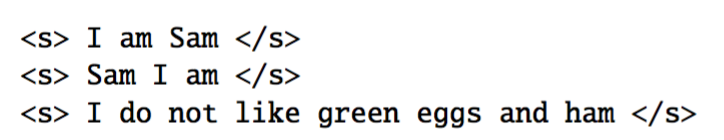
\includegraphics[scale=0.6]{figures/jurafsky-ngram-simple1.png}

the $\textless$s$\textgreater$ indicate start and end tags, they are to be treated just as words. 
It is important to include them to ensure that the probability estimates that we are extracting
are well behaved.

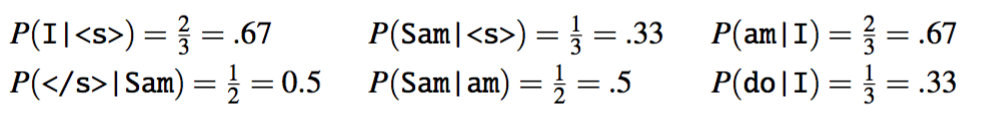
\includegraphics[scale=0.6]{figures/jurafsky-ngram-simple2.png}



\end{frame}
%%%%%%%%%%%%%%%%%%%%%%%%%%%%%%%%%%%%%%%%%%%%%%%%%%%%%%%%%%%%%%%%%%%%%%%%%





%%%%%%%%%%%%%%%%%%%%%%%%%%%%%%%%%%%%%%%%%%%%%%%%%%%%%%%%%%
\begin{frame}[fragile]{Bigram illustration}

\begin{center}
\code{I want to make America great again}
\end{center}
\begin{eqnarray*}
P(\text{I} | \text{\textless start \textgreater }) P(\text{want} | \text{I}) P(\text{to} | \text{want}) P(\text{make} | \text{to})P(\text{America} | \text{make}) \\
P(\text{great} | \text{America}) P(\text{again}|\text{great}) P(\text{\textless end \textgreater } | \text{again})
\end{eqnarray*}
Assume $P(\text{I} | \text{\textless start \textgreater })= 25\%$ and $P(\text{\textless end \textgreater } | \text{again})=25\%.$
\end{frame}
%%%%%%%%%%%%%%%%%%%%%%%%%%%%%%%%%%%%%%%%%%%%%%%%%%%%%%%%%%%%%%%%%%%%%%%%%


%%%%%%%%%%%%%%%%%%%%%%%%%%%%%%%%%%%%%%%%%%%%%%%%%%%%%%%%%%
\begin{frame}[fragile, shrink]{Bigram illustration}
\begin{knitrout}\tiny
\definecolor{shadecolor}{rgb}{0.969, 0.969, 0.969}\color{fgcolor}\begin{kframe}
\begin{verbatim}
##       ngrams estprop         ngrams  estprop
##  1:   to be   0.1108  make america  0.186782
##  2: want to   0.6382        make a  0.146552
##  3:  i dont   0.0797      make our  0.140805
##  4:   to do   0.0696       make it  0.137931
##  5: i think   0.0723 america great  0.269663
##  6:  i mean   0.0614 america first  0.117978
##  7:  i said   0.0611    america is  0.044944
##  8:  i have   0.0609 america shower 0.005618
##  9: to have   0.0403   great again  0.107715
## 10:  to get   0.0386  great people  0.045124
## 11:   i was   0.0420    great with  0.034934
## 12:  i want   0.0404     great and  0.032023
## 13: to make   0.0299      a shower  0.000279
## 14:  to the   0.0271  shower again  1.000000
\end{verbatim}
\end{kframe}
\end{knitrout}
\begin{eqnarray*}
P(\text{I} | \text{\textless start \textgreater }) P(\text{want} | \text{I}) P(\text{to} | \text{want}) P(\text{make} | \text{to}) P(\text{America} | \text{make}) \\
P(\text{great} | \text{America}) P(\text{again}|\text{great})  P(\text{\textless end \textgreater } | \text{again})\\
= 0.25 x 0.04 x 0.64 x 0.03 x 0.19 x 0.27 x 0.11 x 0.25 = 0.0000002708
\end{eqnarray*}
\begin{eqnarray*}
P(\text{I} | \text{\textless start \textgreater }) P(\text{want} | \text{I}) P(\text{to} | \text{want}) P(\text{make} | \text{to}) P(\text{America} | \text{make}) \\
P(\text{\textbf{shower}} | \text{America}) P(\text{again}|\text{\textbf{shower}}) P(\text{\textless end \textgreater } | \text{again})\\
= 0.25 x 0.04 x 0.64 x 0.03 x 0.19 x 0.0056179775 x 1 x 0.25 = 0.00000005123
\end{eqnarray*}
\end{frame}
%%%%%%%%%%%%%%%%%%%%%%%%%%%%%%%%%%%%%%%%%%%%%%%%%%%%%%%%%%%%%%%%%%%%%%%%%


%%%%%%%%%%%%%%%%%%%%%%%%%%%%%%%%%%%%%%%%%%%%%%%%%%%%%%%%%%
\begin{frame}[fragile]{What do we learn?}

\begin{itemize}

\item N-gram models capture syntatic features and general knowledge (here, knowledge about the underlying speeker)

\item It turns out that linguistic features such as word sequences ``I want'' are reasonably frequent and they capture linguistic features: verbs tend to follow subject as indicated by ``I''.

\item ``america shower'' is much more rare in Trump's speeches compared to ``america great''.

\item N-gram models can be trained by counting and normalization

\end{itemize}


\end{frame}
%%%%%%%%%%%%%%%%%%%%%%%%%%%%%%%%%%%%%%%%%%%%%%%%%%%%%%%%%%%%%%%%%%%%%%%%%



%%%%%%%%%%%%%%%%%%%%%%%%%%%%%%%%%%%%%%%%%%%%%%%%%%%%%%%%%%
\begin{frame}[fragile,shrink]{Illustration of estimating N-Gram probabilities.}

We will use Maximum Likelihood estimation, illustrate and proof what is the maximum likelihood estimator using a unigram model 

$$P(w_1,..., w_n) = \prod_{k=1}^{n}{P(w_k)} $$

This can think of this as a sequence of independent \emph{Bernoulli} trials with success probability $p_k$ for word $k$.

Suppose you observe a sample of size $N$ of word sequences of length $n$, $\{W^1, ..., W^N\}$. So each $W^i = (w_{i1},..., w_{in})$, where $w_{ij} = 1$ in case word $w_j$ is present in sequence $i$.

What is the likelihood of observing a specific sequence?

$$P(W^i) = \prod_{k=1}^{n}{p_k^{w_{ik}}(1-p_k)^{1-w_{ik}} }$$

What is the likelihood of observing the whole sample?

$$\prod_{i=1}^{N} P(W^i) = \prod_{i=1}^{N}\prod_{k=1}^{n}{p_k^{w_{ik}}(1-p_k)^{1-w_{ik}} }$$


\end{frame}
%%%%%%%%%%%%%%%%%%%%%%%%%%%%%%%%%%%%%%%%%%%%%%%%%%%%%%%%%%%%%%%%%%%%%%%%%


%%%%%%%%%%%%%%%%%%%%%%%%%%%%%%%%%%%%%%%%%%%%%%%%%%%%%%%%%%
\begin{frame}[fragile,shrink]{Log Likelihood}

Taking logs
$$\sum_{i=1}^{N}\sum_{k=1}^{n}{w_{ik} log(p_k)} + (1-w_{ik}) log(1-p_k) $$

We want to find optimal $p_1, ..., p_n$, so take FOC. Notice that everything is additive and there are no interactions between individual $p_k$. Take FOC with respect to $p_k$.

$$\sum_{i=1}^{N} \frac{1}{p_k} w_{ik} - \sum_{i=1}^{N}  (1-w_{ik}) \frac{1}{1-p_k} = 0$$

This yields

$$p_k = \frac{\sum_{i=1}^{N} w_{ik}}{N} \quad \forall k $$

where the numerator is just the number of word sequences that contain the word and $N$ is just the sample size. 
\end{frame}
%%%%%%%%%%%%%%%%%%%%%%%%%%%%%%%%%%%%%%%%%%%%%%%%%%%%%%%%%%%%%%%%%%%%%%%%%



%%%%%%%%%%%%%%%%%%%%%%%%%%%%%%%%%%%%%%%%%%%%%%%%%%%%%%%%%%
\begin{frame}[fragile]{In case of Bigram model}
For Bigram model, the intuitive way to estimate the probability $P(w_k| w_{k-1})$ is to get the counts of word sequences $C(w_{k-1}, w_k)$ from a corpus and normalize this by the counts of word that share the same first word, i.e. we estimate

$$P(w_k|w_{k-1}) = \frac{C(w_{k-1},w_k)}{\sum_{w}{C(w_{k-1},w)}} = \frac{C(w_{k-1},w_k)}{C(w_{k-1})}$$

Note that $\sum_{w}{C(w_{k-1},w)} = C(w_{k-1})$

I.e. the number of word pairs that share the starting word $w_{k-1}$ should simply add up to the number of times the word $w_{k-1}$ appears.

\end{frame}
%%%%%%%%%%%%%%%%%%%%%%%%%%%%%%%%%%%%%%%%%%%%%%%%%%%%%%%%%%%%%%%%%%%%%%%%%



%%%%%%%%%%%%%%%%%%%%%%%%%%%%%%%%%%%%%%%%%%%%%%%%%%%%%%%%%%
\begin{frame}[fragile]{A Bigram Example}
\begin{center}
\code{I want to make America great again}
\end{center}
\begin{knitrout}\small
\definecolor{shadecolor}{rgb}{0.969, 0.969, 0.969}\color{fgcolor}\begin{kframe}
\begin{verbatim}
##          i want  to make america great again
## i        2  196   0    3       0     0     0
## want     5    0 485    0       0     0     0
## to       5    4   0  163       0     1     0
## make     0    0   0    0      65    17     0
## america  1    0   4    0       0    48     1
## great   16    0   7    0       0    14    74
## again   19    0   3    0       1     0     0
\end{verbatim}
\end{kframe}
\end{knitrout}
Normalization: divide each row's counts by appropriate unigram counts for $w_{n-1}$
\begin{knitrout}\small
\definecolor{shadecolor}{rgb}{0.969, 0.969, 0.969}\color{fgcolor}\begin{kframe}
\begin{verbatim}
##    [,1]   [,2]   [,3]   [,4]    [,5]   [,6]      [,7]   
## X1 "to"   "want" "i"    "great" "make" "america" "again"
## V1 "5460" " 760" "4857" " 687"  " 348" " 178"    " 246"
\end{verbatim}
\end{kframe}
\end{knitrout}
\end{frame}
%%%%%%%%%%%%%%%%%%%%%%%%%%%%%%%%%%%%%%%%%%%%%%%%%%%%%%%%%%%%%%%%%%%%%%%%%


%%%%%%%%%%%%%%%%%%%%%%%%%%%%%%%%%%%%%%%%%%%%%%%%%%%%%%%%%%
\begin{frame}[fragile]{A Bigram Example}

\begin{knitrout}\tiny
\definecolor{shadecolor}{rgb}{0.969, 0.969, 0.969}\color{fgcolor}\begin{kframe}
\begin{verbatim}
##                i     want     to     make america    great   again
## i       0.000412 0.040354 0.0000 0.000618 0.00000 0.000000 0.00000
## want    0.006579 0.000000 0.6382 0.000000 0.00000 0.000000 0.00000
## to      0.000916 0.000733 0.0000 0.029853 0.00000 0.000183 0.00000
## make    0.000000 0.000000 0.0000 0.000000 0.18678 0.048851 0.00000
## america 0.005618 0.000000 0.0225 0.000000 0.00000 0.269663 0.00562
## great   0.023290 0.000000 0.0102 0.000000 0.00000 0.020378 0.10771
## again   0.077236 0.000000 0.0122 0.000000 0.00407 0.000000 0.00000
\end{verbatim}
\end{kframe}
\end{knitrout}
\begin{itemize}
\item Ratio of $\frac{C(w_n, w_{n-1})}{C(w_{n-1})}$ is a maximum Likelihood estimate for $P(w_n|w_{n-1})$

\item We observe that many raw counts are zero: the matrix is sparse.

\item The larger $N$, the more sparse will these matrices get.

\item However, larger $N$ generally results in better performance as more history is incorporated.
\end{itemize}
\end{frame}
%%%%%%%%%%%%%%%%%%%%%%%%%%%%%%%%%%%%%%%%%%%%%%%%%%%%%%%%%%%%%%%%%%%%%%%%%


%%%%%%%%%%%%%%%%%%%%%%%%%%%%%%%%%%%%%%%%%%%%%%%%%%%%%%%%%%
\begin{frame}[fragile,shrink]{Trade-off: Higher order N-gram versus lower order N-grams}
Unigram Trump Babbler
\begin{knitrout}\tiny
\definecolor{shadecolor}{rgb}{0.969, 0.969, 0.969}\color{fgcolor}\begin{kframe}
\begin{verbatim}
## [1] "prosperity not talking about the game and more you mean but ill tell you know shes going t"
## [2] "o terminate obamacare with a lot its deadly totally destabilized the worst human being tre"
## [3] "ated me so im not smart and tell you get on trade agreement you look we have to end "
\end{verbatim}
\end{kframe}
\end{knitrout}
Bigram Trump Babbler
\begin{knitrout}\tiny
\definecolor{shadecolor}{rgb}{0.969, 0.969, 0.969}\color{fgcolor}\begin{kframe}
\begin{verbatim}
## [1] "from pakistan and he was talking to some place it costs 3 billion and i said ok then i hav"
## [2] "e to happen with these two nations and must regard them with their families we mourn as on"
## [3] "e united people with force purpose and determination but the muslims living in this "
\end{verbatim}
\end{kframe}
\end{knitrout}
Trigram Trump Babbler
\begin{knitrout}\tiny
\definecolor{shadecolor}{rgb}{0.969, 0.969, 0.969}\color{fgcolor}\begin{kframe}
\begin{verbatim}
## [1] "permanently admits more than 100000 immigrants from the middle east our government has bee"
## [2] "n admitting ever growing numbers year after year without any effective plan for our own se"
## [3] "curity in fact clintons state department was in charge of admissions and the admissions pr"
## [4] "ocess for people applying to enter from overseas "
\end{verbatim}
\end{kframe}
\end{knitrout}
Quadrigram Trump Babbler
\begin{knitrout}\tiny
\definecolor{shadecolor}{rgb}{0.969, 0.969, 0.969}\color{fgcolor}\begin{kframe}
\begin{verbatim}
## [1] "tough as nails hes going to be your champion im going to be good for womens health issues "
## [2] "its very important to me it was instructional when i did the art of the deal pac after the"
## [3] " book they have all these pacs and the money comes in and its "
\end{verbatim}
\end{kframe}
\end{knitrout}
as $N$ increases, the number of parameters to be estimated explodes. In addition, as we have seen, the matrices are very sparse - many zeroes!
\end{frame}
%%%%%%%%%%%%%%%%%%%%%%%%%%%%%%%%%%%%%%%%%%%%%%%%%%%%%%%%%%%%%%%%%%%%%%%%%

%%%%%%%%%%%%%%%%%%%%%%%%%%%%%%%%%%%%%%%%%%%%%%%%%%%%%%%%%%
\begin{frame}[fragile]{Curse of Dimensionality of N-gram model}

Suppose you have a vocabulary of size $|V|$. Assuming no constraints imposed by language structure. How many different conditional probabilites are there to estimate?

\begin{itemize}

\item There are $|V|$ sentences, containing exactly 1 words.

\item There are $|V| \times |V|$ sentences containing 2 words

\item There are $|V| \times |V| \times |V|$ sentences containing 3 words

\end{itemize}

In total there are $|V|^{N}$  parameters in an n-gram for vocabulary size $|V|$.

\end{frame}
%%%%%%%%%%%%%%%%%%%%%%%%%%%%%%%%%%%%%%%%%%%%%%%%%%%%%%%%%%%%%%%%%%%%%%%%%



%%%%%%%%%%%%%%%%%%%%%%%%%%%%%%%%%%%%%%%%%%%%%%%%%%%%%%%%%%
\begin{frame}[fragile]{Uses of N-gram models for language categorization}

\url{https://www.let.rug.nl/~vannoord/TextCat/textcat.pdf}

\end{frame}
%%%%%%%%%%%%%%%%%%%%%%%%%%%%%%%%%%%%%%%%%%%%%%%%%%%%%%%%%%%%%%%%%%%%%%%%%


%%%%%%%%%%%%%%%%%%%%%%%%%%%%%%%%%%%%%%%%%%%%%%%%%%%%%%%%%%
\begin{frame}[fragile]{Babbling Donald Trump}
\begin{knitrout}\tiny
\definecolor{shadecolor}{rgb}{0.969, 0.969, 0.969}\color{fgcolor}\begin{kframe}
\begin{alltt}
\hlkwd{library}\hlstd{(ngram)}
\hlstd{TRUMP} \hlkwb{<-} \hlkwd{readLines}\hlstd{(}\hlkwc{con} \hlstd{=} \hlstr{"../../Data/Trump-Speeches.txt"}\hlstd{)}
\hlcom{# concatenate into one massive string, remove empty lines}
\hlstd{TRUMP} \hlkwb{<-} \hlstd{TRUMP[}\hlopt{-}\hlkwd{grep}\hlstd{(}\hlstr{"^SPEECH|^$"}\hlstd{, TRUMP)]}
\hlstd{TRUMP} \hlkwb{<-} \hlkwd{gsub}\hlstd{(}\hlstr{" +"}\hlstd{,} \hlstr{" "}\hlstd{, TRUMP)}
\hlstd{TRUMP} \hlkwb{<-} \hlkwd{paste}\hlstd{(TRUMP,} \hlkwc{collapse} \hlstd{=} \hlstr{" "}\hlstd{)}
\hlstd{TRUMP} \hlkwb{<-} \hlkwd{ngram}\hlstd{(TRUMP,} \hlkwc{n} \hlstd{=} \hlnum{3}\hlstd{)}
\hlkwd{str_break}\hlstd{(}\hlkwd{babble}\hlstd{(TRUMP,} \hlkwc{genlen} \hlstd{=} \hlnum{35}\hlstd{,} \hlkwc{seed} \hlstd{=} \hlnum{130}\hlstd{))}
\end{alltt}
\begin{verbatim}
## [1] "I have as big a heart as anybody. We want to win Iowa, folks. Because look, I love the poo"
## [2] "rly educated. We’re the smartest people, we’re the most loyal people by far. Everybody say"
## [3] "s it. "
\end{verbatim}
\end{kframe}
\end{knitrout}

\end{frame}
%%%%%%%%%%%%%%%%%%%%%%%%%%%%%%%%%%%%%%%%%%%%%%%%%%%%%%%%%%%%%%%%%%%%%%%%%

\end{document}

